\chapter{Parametric study of a flow around a cylinder}
	\label{eulerVerification}
	In the following chapter we will regard a flow at Mach $0.2$ around a frictionless cylinder with adiabatic slip walls at changing parameters such as the polynomial degree, the mesh size and the position of the cylinder in order to validate \gls{bosss} with immersed boundaries concerning robustness and convergence.

	\section{Robustness study}
	In the first study regarding the frictionless cylinder, we compare the absolute error of entropy for a polynomial degree from $1$ to $3$ along a shift of the centre point of the cylinder from $-0.075$ to $0.075$ at steps of $0.015$. By shifting the cylinder we can consider several cases where the cells would be cut differently and therefore cause different cell agglomerations. The cell agglomeration threshold is at a constant level of $0.5$ in a mesh of $32 \times 32$ cells. In this example we aim at proving the robustness of the solver as for each position of the cylinder the error of entropy should not vary too much thus making it independent of the way the border cells are cut. \\ \\

	\begin{figure}[htp]	
		\centering
		\begin{tikzpicture}
			\begin{semilogyaxis}[xlabel ={Position of Centre Point of the Cylinder}, ylabel ={$L_2$ Error of Entropy}, grid =major, legend entries ={$P=1$,$P=2$, $P=3$}, unbounded coords=jump, legend style = {cells = {anchor=east}, legend pos=outer north east,}, scaled x ticks = false]
				\addplot table[ x =shift, y =error1] {data/shift.dat};
				\addplot table[ x =shift, y =error2] {data/shift.dat};
				\addplot table[ x =shift, y =error3] {data/shift.dat};
			\end{semilogyaxis}	
		\end{tikzpicture}
		\label{shifterror}	
		\caption{Convergence Plot}
	\end{figure}
	

	As we look at the chart \ref{shifterror}, first of all we will note that the absolute error of entropy decreases with increasing polynomial degree. As a higher polynomial degree implies a better approximation this can be explained very easily. \\ \indent
	Secondly, we can observe that the error of entropy behaves roughly symmetrically to the ordinate. As we shifted the cylinder symmetrically this observation does not surprise us either. \\ \indent
	Regarding the absolute error at a polynomial degree of 3, it is striking that this curve shows a much higher error difference compared to degrees 1 and 2. There are two peaks at a shift of $\pm 0.03$; these discordant values where produced because the calculation stopped early. Unlike all other cases during this study, the calculation did not stop because the convergence criterion (change of error of entropy $\leq 10^{-13}$) was reached but because the CFL number got invalid.\\ \indent
	As these two values rather count as exceptions, we now consider two cases with a degree of $2$ at the shifts of $-0.06$ and $-0.03$. \\\\
	
	\begin{figure}[htp]
		\centering
		\begin{subfigure}[b]{0.5\textwidth}
			\centering
			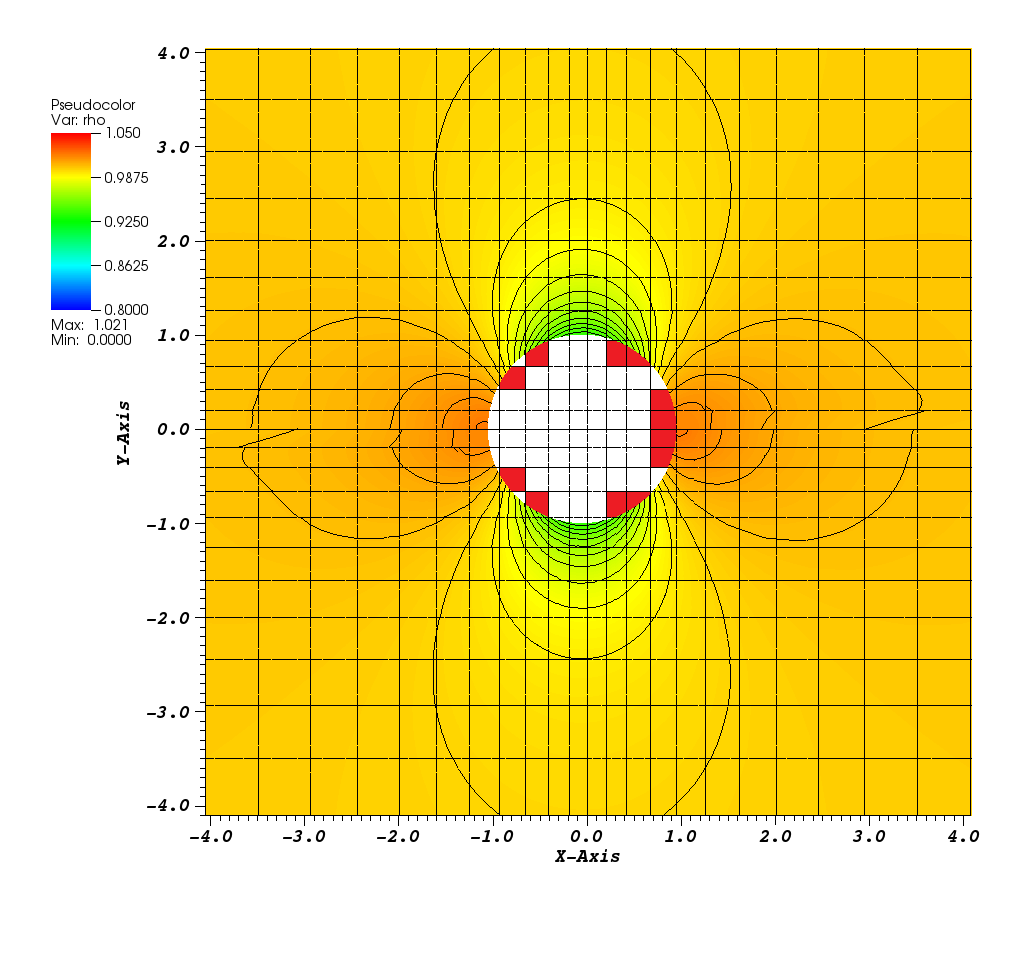
\includegraphics[height=8cm]{2_2.PNG}
			\caption{Degree 2, shift $-0.06$}
			\label{fig:2_2}
		\end{subfigure}%
		\begin{subfigure}[b]{0.5\textwidth}
			\centering
			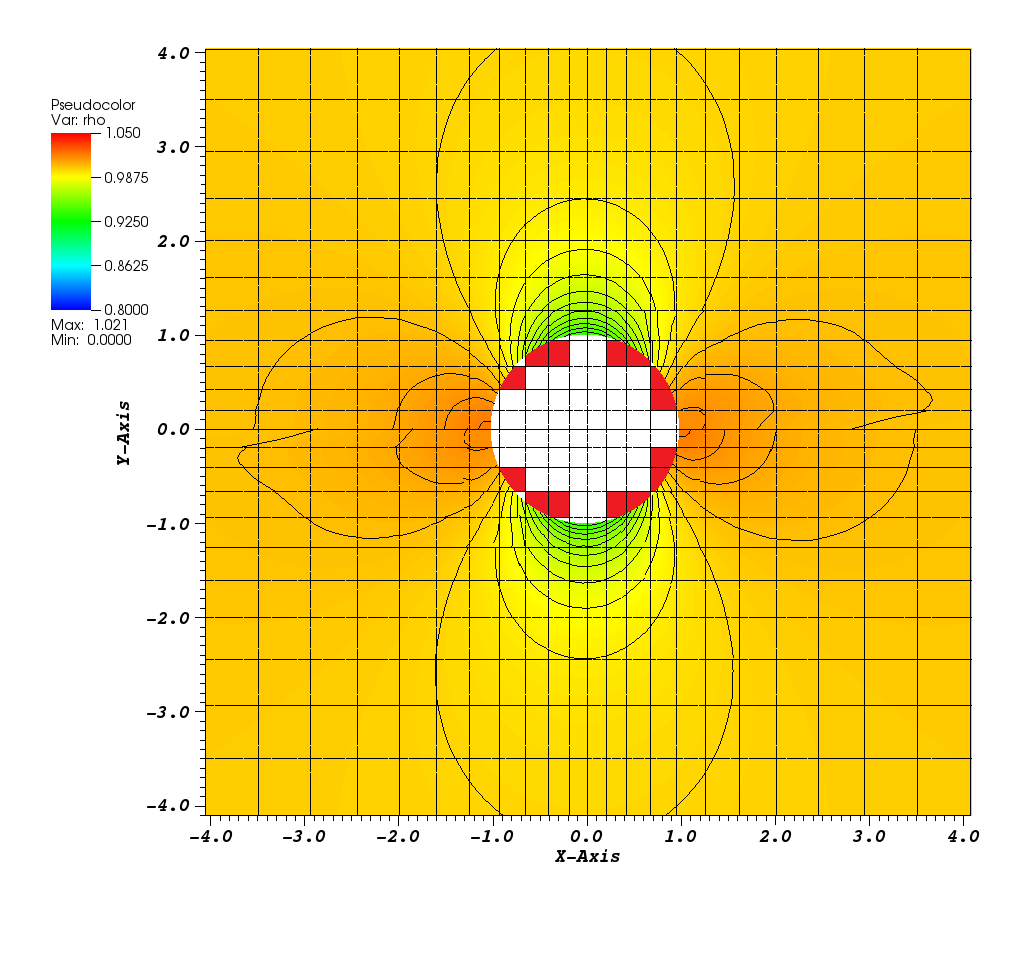
\includegraphics[height=8cm]{2_4.PNG}
			\caption{Degree 2, shift $-0.03$}
			\label{fig:2_4}
		\end{subfigure}
		\caption{Isolines of pressure}\label{fig:isoshift}
	\end{figure}
	
	In figure \ref{fig:isoshift} you can see the two mentioned cases with highlighted isolines of pressure and pseudocolored density. As only the upper half of the cylinder has been calculated, I reflected the results through the centre point of the cylinder. Therefore you can easily see that the results are not correct, as the flow before and after the obstacle should be identical. Furthermore you can see that in \ref{fig:2_2} the isolines are smoother than in \ref{fig:2_4}. In order to give an explanation for the higher error of entropy in \ref{fig:2_4} I highlighted the cells that should have been agglomerated in red. In the left case there are less agglomerated cells than in the right one, therefore there was a not so big agglomeration mistake made.\\\\
	
	Except for the two discordant values at polynomial degree $3$, the error of entropy changes very little for the different cases. We can therefore assume that the solver is good enough validated concerning the way the agglomerated cells influence the calculation. \todo{cases nochmal rechnen um peaks wegzukriegen}
	
	\section{Convergence study of mesh size and polynomial degree}
	
	In the second study we vary the mesh size of our geometry from $32 \times 32$ by $64 \times 64$ to $128 \times 128$ cells. Additionally we also vary the polynomial degree from $0$ to $4$, consequently regarding fifteen cases in total. \\
	Our aim is the verification of the convergence of the RKDGM based solver for the inviscid cylinder. Therefore we hope to achieve an experimental order of convergence that is near the optimal rate $O(h^{P+1})$. In chart \ref{mesherror} I compared the absolute error entropy to the mesh size logarithmically for each polynomial degree. 	
	\begin{figure}[htp]
		\centering		
		\begin{tikzpicture}
			\begin{loglogaxis}[xlabel ={Cells per Direction}, ylabel ={$L_2$ Error of Entropy}, grid =major, legend entries ={$P=0$,$P=1$,$P=2$, $P=3$, $P=4$}, unbounded coords=jump, legend style = {cells = {anchor=east}, legend pos=outer north east,} ]
				\addplot table[ x =meshSize, y =error0] {data/test.dat};
				\addplot table[ x =meshSize, y =error1] {data/test.dat};
				\addplot table[ x =meshSize, y =error2] {data/test.dat};
				\addplot table[ x =meshSize, y =error3] {data/test.dat};
				\addplot table[ x =meshSize, y =error4] {data/test.dat};
			\end{loglogaxis}	
		\end{tikzpicture}
		\label{mesherror}	
		\caption{Convergence Plot}
	\end{figure}

	As you can see in \ref{mesherror} each graph has a more or less constant gradient that is higher with increasing polynomial degree which is approximately of the order $P+1$ as we hoped. Regarding the values of the $128 \times 128$ mesh there are two discordant values: the case with mesh size $128 \times 128$ and polynomial degree $P = 4$ did not terminate due to the error of entropy residual but because the CFL number could not be determined and therefore no value for the error of entropy was computed. The case for $P = 3$ has a disproportionately high value that is caused by two cells as can be seen in \ref{fig:case14detail}. In order to correct the value I changed the \textit{node count safety factor} from $2$ to $5$ which increases the robustness and therefore lets the calculation finish due to the residual. In \ref{fig:case14} you can see the visualised flow of the inspected case with the critical spot where entropy is produced in \ref{fig:case14detail} and the flow after the correction in \ref{fig:case14detailneu}. Please remark that differently coloured entropy ranges had to be used in the two cases in order to point out the critical cell in \ref{fig:case14detail}.
	

	\begin{figure}[htp]
		\centering
		\begin{subfigure}[b]{0.3\textwidth}
			\centering
			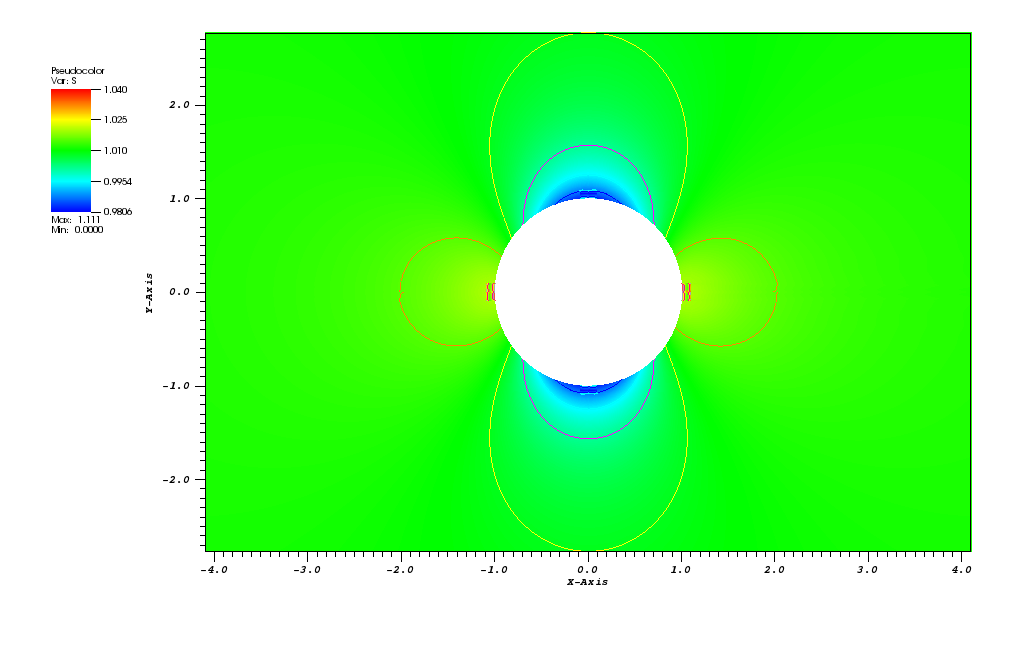
\includegraphics[height=3.3cm]{case14.PNG}
			\caption{Overview of flow before correction}
			\label{fig:case14groß}
		\end{subfigure}%
		\begin{subfigure}[b]{0.3\textwidth}
			\centering
			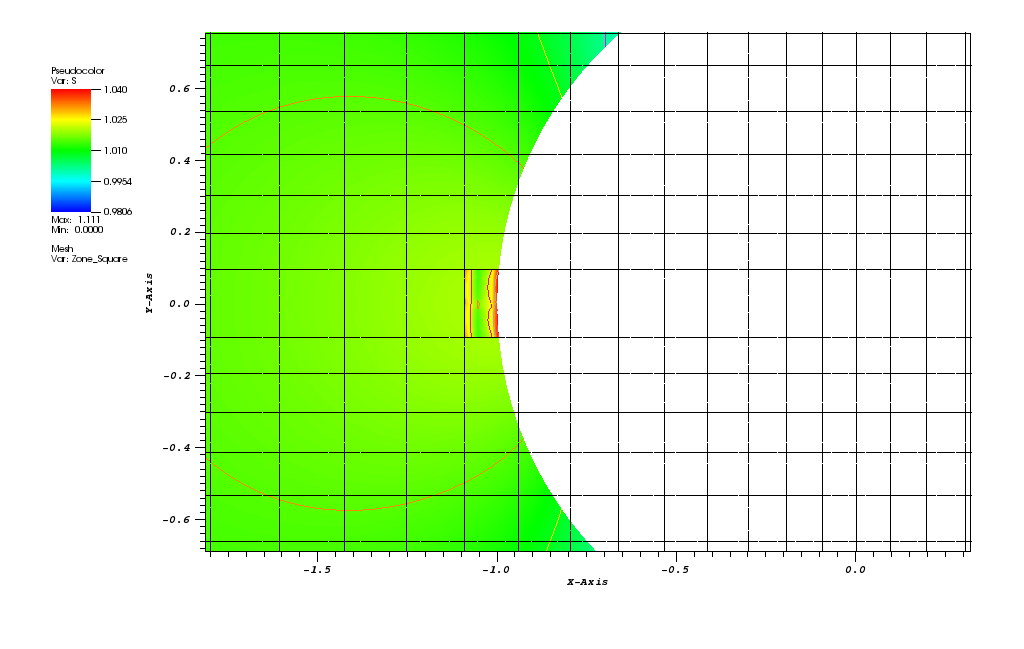
\includegraphics[height=3.3cm]{case14komisch.PNG}
			\caption{Detailed view of critical cell before correction}
			\label{fig:case14detail}
		\end{subfigure}
		\begin{subfigure}[b]{0.3\textwidth}
			\centering
			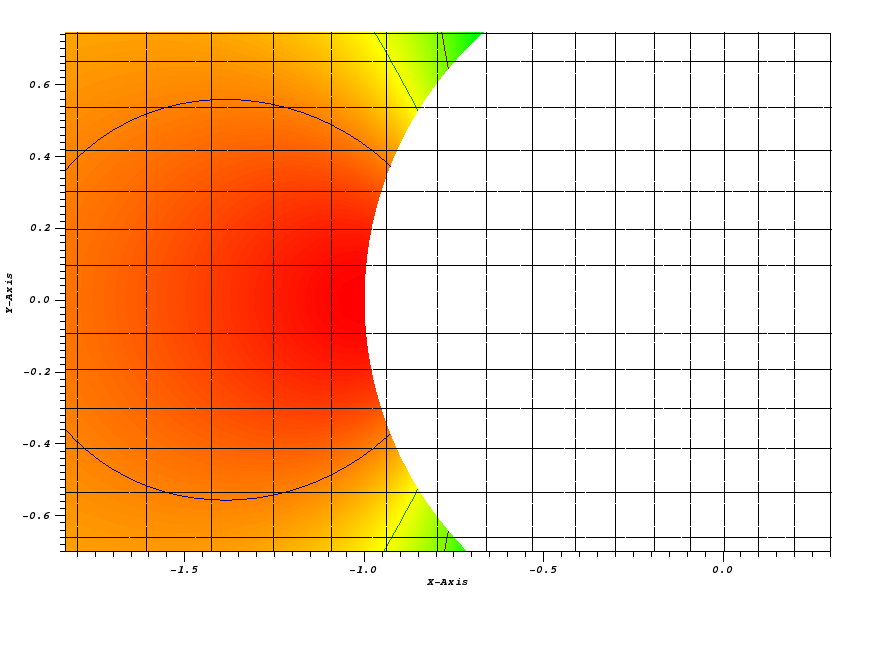
\includegraphics[height=3.3cm]{case14normal.PNG}
			\caption{Detailed view of critical cell after correction}
			\label{fig:case14detailneu}
		\end{subfigure}
		\caption{Mesh size $128 \times 128$, $P = 3$}
		\label{fig:case14}
	\end{figure}
	
	Concluding, we remark that the convergence behaves as desired with an order close to the optimal rate of $O(h^{P+1})$. Nevertheless to receive the correct result it should always be guaranteed that the calculation stops due to the residual rather than illegal values for momentum even if that means heightening the overall runtime by increasing the node count safety factor thus robustness.
	
